\subsection*{Модель сегрегации Шеллинга в Python}
\addcontentsline{toc}{subsection}{Модель сегрегации Шеллинга в Python}

\textbf{Задание:}\\
Реализовать модель сегрегации Шеллинга в Python.\\

\textbf{Решение:}\\
Суть данного алгоритма была описана в предыдущем разделе. Здесь же будет рассмотрена просто реализация предыдущей задачи на языке программирования Python.\\

Для начала был создан класс \textit{Person}, который содержит информацию о члене популяции. У него имеется два поля: тип и счастлив ли данный агент или нет. (Рисунок \ref{fig:scheling_python1})
\begin{figure}[h]
	\centering 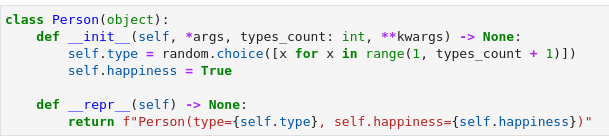
\includegraphics[scale=0.5]{scheling_python1}
	\caption{Класс члена популяции \textit{Person}}
	\label{fig:scheling_python1}
\end{figure}

Далее был создан класс популяции -- \textit{Population}, в котором изначально генерировалась популяция агентов и задавалась начальная конфигурация системы. (Рисунок \ref{fig:scheling_python2})
\begin{figure}[h]
	\centering 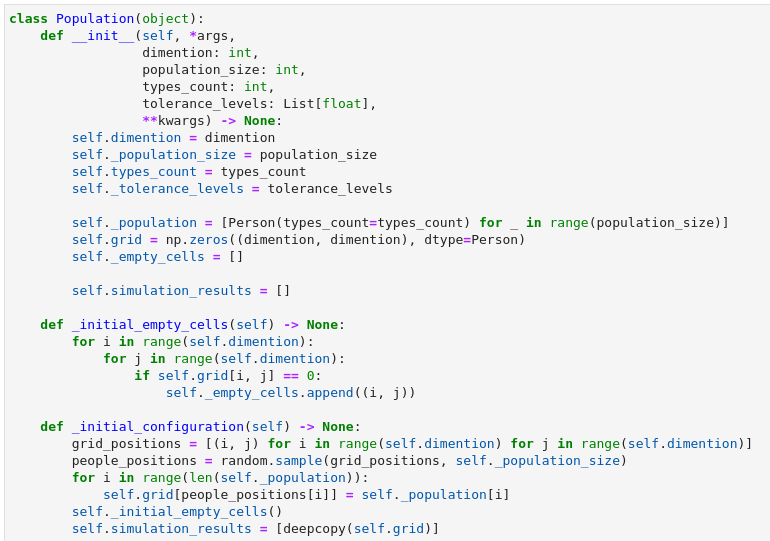
\includegraphics[scale=0.4]{scheling_python2}
	\caption{Класс популяции \textit{Population}}
	\label{fig:scheling_python2}
\end{figure}

\newpage

Далее были созданы функции для перемещения агента в системе, изменения уровня счастья конкретного агента и собственно основной функции симуляции. (Рисунок \ref{fig:scheling_python3})
\begin{figure}[h]
	\centering 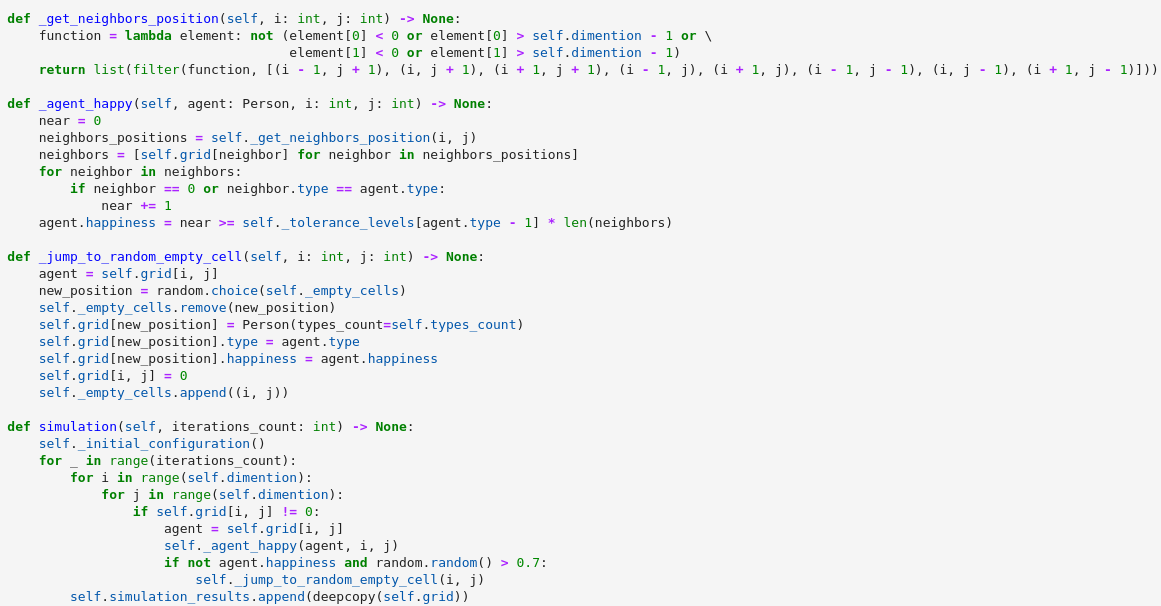
\includegraphics[scale=0.4]{scheling_python3}
	\caption{Функции для перемещения агентов в системе и симуляции}
	\label{fig:scheling_python3}
\end{figure}

Также были созданы вспомогательные функции для отрисовки текущего состояния системы и для анимации получившихся результатов. (Рисунок \ref{fig:scheling_python4})
\begin{figure}[h]
	\centering 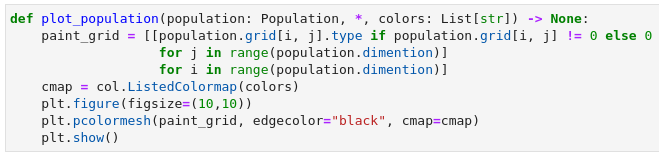
\includegraphics[scale=0.5]{scheling_python4}
	\caption{Функции для отрисовки текущего состояния системы}
	\label{fig:scheling_python4}
\end{figure}

\newpage

\begin{figure}[h]
	\centering 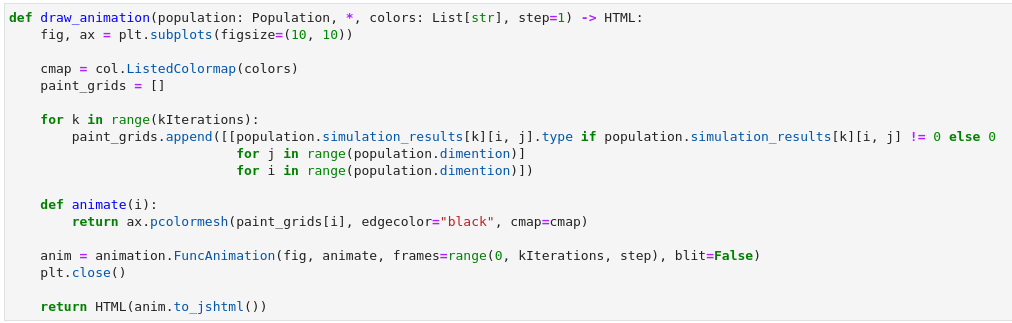
\includegraphics[scale=0.5]{scheling_python5}
	\caption{Функции для анимации процесса симуляции}
	\label{fig:scheling_python5}
\end{figure}

Ещё были реализованы функции для сбора статистики по популяции, а именно отслеживание количества счастливых агентов. (Рисунок \ref{fig:scheling_python6})

\begin{figure}[h]
	\centering 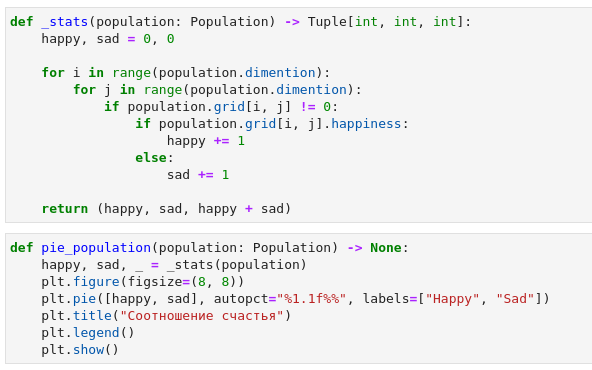
\includegraphics[scale=0.5]{scheling_python6}
	\caption{Функции сбора статистики по популяции}
	\label{fig:scheling_python6}
\end{figure}

\newpage

Визуализация различных уровней счастья агентов в модели, построенной при помощи Python, сходна с той, что была получена при использовании среды AnyLogic. (Рисунок \ref{fig:scheling_python7})

\begin{figure}[h]
	\centering 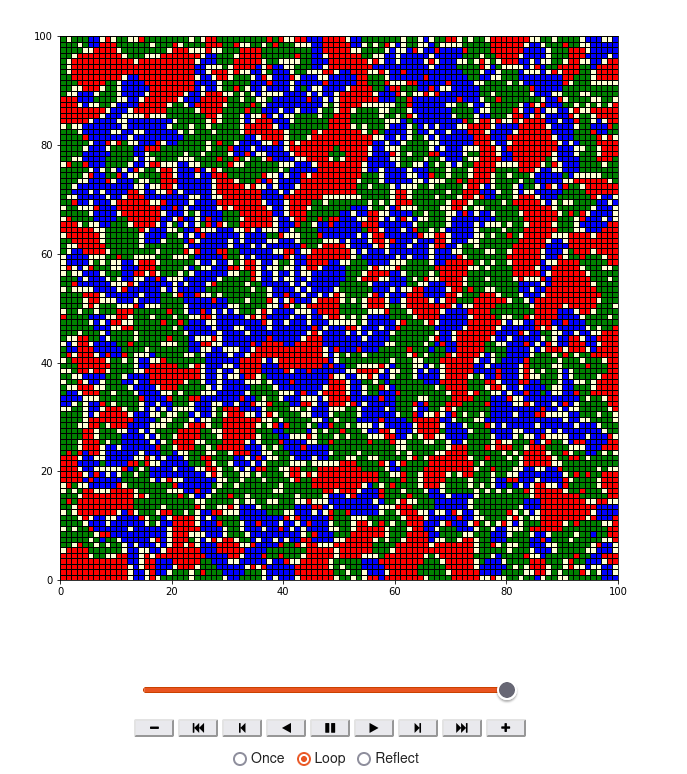
\includegraphics[scale=0.3]{scheling_python7}
	\caption{Визуализация полученных результатов}
	\label{fig:scheling_python7}
\end{figure}

\begin{figure}[h]
	\centering 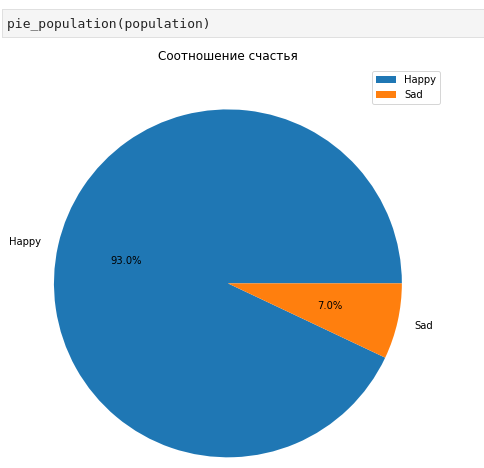
\includegraphics[scale=0.3]{scheling_python8}
	\caption{Статистика по полученным результатам}
	\label{fig:scheling_python8}
\end{figure}

Также были промоделированы различные другие ситуации, допустим когда рассматривается всего две типа людей или когда изменяется уровень толерантности групп.\\

Таким образом, была реализована модель сегрегации Шеллинга при различных условиях взаимодействия агентов.